\chapter{Studi Literatur}
\label{chapter:studi-literatur}

Bab ini akan diisi oleh studi literatur yang terkait dengan topik persoalan pada tugas akhir untuk memberikan informasi mengenai dasar teori dan literatur yang digunakan. Bab ini diharapkan dapat membantu pembaca memiliki pengetahuan yang menyeluruh dan dasar yang cukup untuk mengerti penelitian ini.

\section{Blockchain}
\label{sec:blockchain}

\subsection{Konsep dan Struktur Blockchain}
\label{subsec:konsep-struktur-blockchain}

Blockchain adalah sebuah sistem pencatatan data terdistribusi yang tersusun atas serangkaian blok, di mana setiap blok menyimpan daftar transaksi secara lengkap seperti \textit{public ledger} konvensional. Data disimpan secara terdistribusi pada banyak \textit{node} dalam jaringan, sehingga tidak ada entitas terpusat yang mengontrol keseluruhan sistem. Setiap blok yang memuat transaksi harus divalidasi menggunakan mekanisme konsesus tertentu sebelum ditambahkan ke dalam rantai blok. Proses konsensus melibatkan mayoritas dari \textit{node} untuk menyetujui atau menolak \textit{state} baru dari \textit{ledger}, sehingga menjamin integritas dan keaslian dari data \parencite{zheng2018blockchain,nofer2017blockchain}.

Pada sistem Blockchain klasik, setiap blok umumnya memiliki daftar transaksi yang lengkap, ditambah dengan \textit{timestamp} pembuatan blok, nilai \textit{hash} dari blok sebelumnya ("\textit{parent}"), dan sebuah \textit{nonce}, yang adalah sebuah angka acak yang digunakan untuk mekanisme verifikasi \textit{hash}. 
Konsep ini memastikan integritas dari Blockchain dimulai dari blok pertama ("\textit{genesis block}") sampai ke blok terakhir yang akan terus bertambah, karena setiap perubahan data akan membuat nilai \textit{hash} dari sebuah blok berubah, yang harus dipropagasikan ke setiap blok setelahnya.

Aspek penting dari sebuah Blockchain adalah proses konsensus yang dimilikinya, yang dilakukan dengan mengikuti sebuah kumpulan aturan dan prosedur untuk mempertahankan himpunan fakta yang koheren diantara beberapa \textit{participating nodes}. Terdapat banyak mekanisme konsensus yang berbeda yang digunakan dalam \textit{Blockchain network} yang berbeda. Dalam kasus \textit{Bitcoin}, \textit{ledger} yang dianggap \textit{ledger} yang \textit{valid} adalah \textit{ledger} dengan \textit{chain} terpanjang (\textit{longest chain}) \parencite{swanson2015consensus}.

\begin{figure}[ht]
	\centering
	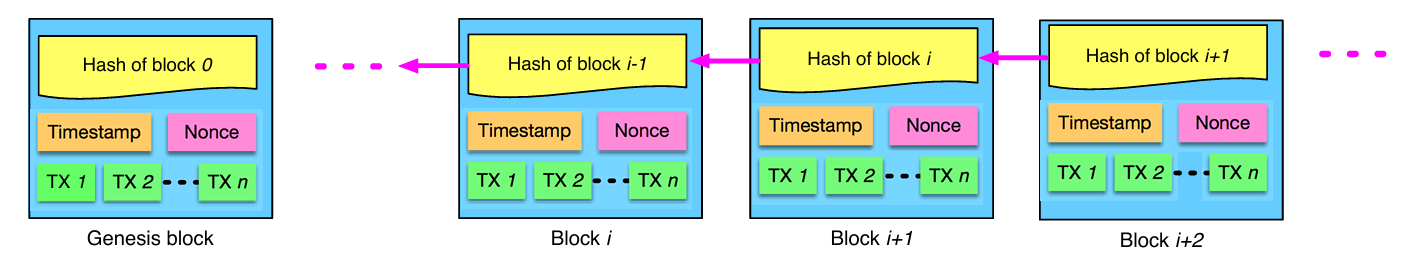
\includegraphics[width=1\textwidth]{resources/chapter-2/struktur-blockchain.png}
	\caption{Struktur blok di dalam Blockchain \parencite{zheng2018blockchain}}
	\label{image:struktur-blockchain}
\end{figure}

Struktur klasik dari sebuah blok pada Blockchain terdiri dari \textit{block header} dan \textit{block body} seperti pada Gambar \ref{image:struktur-blok}. Secara spesifik, \textit{block header} terdiri dari:

\begin{enumerate}
	\item \textit{Block Version}: mengindikasikan set dari aturan validasi yang diikuti.
	\item \textit{Parent Block Hash}: 256-bit \textit{hash} dari blok sebelumnya.
	\item \textit{Merkle Tree Root}: hasil \textit{hash} dari seluruh transaksi pada blok menggunakan mekanisme \textit{Merkle Tree}.
	\item \textit{Timestamp}: \textit{timestamp} saat ini dalam detik sejak 1970-01-01T00:00 UTC.
	\item \textit{nBits}: target \textit{hash} saat ini dalam format \textit{compact}.
	\item \textit{nonce}: \textit{number used only once}, sebuah angka yang digunakan untuk menambahkan tingkat keacakan dari nilai \textit{hash}.
\end{enumerate}

\begin{figure}[ht]
	\centering
	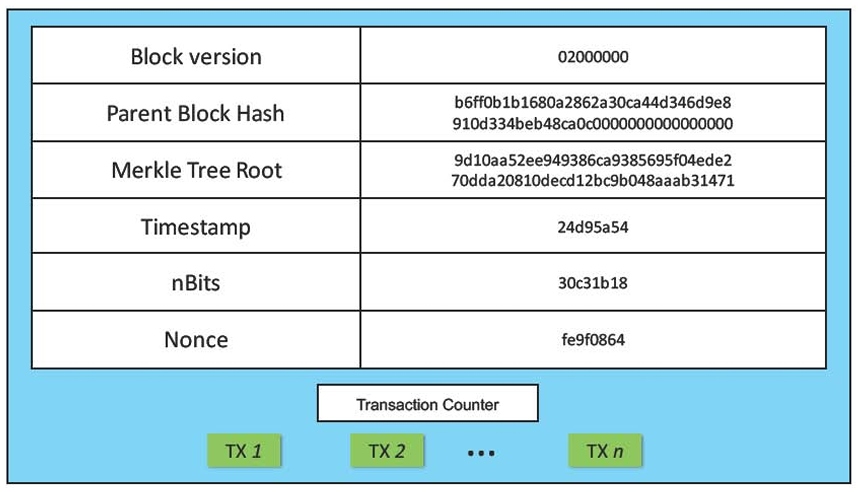
\includegraphics[width=0.7\textwidth]{resources/chapter-2/struktur-block.png}
	\caption{Struktur blok \parencite{zheng2018blockchain}}
	\label{image:struktur-blok}
\end{figure}

\subsection{Karakteristik Blockchain}
\label{subsec:karakteristik-blockchain}

Implementasi dari Blockchain memunculkan karakteristik dari Blockchain itu sendiri. Karakteristik ini dapat muncul secara inheren dari sistem dasar di mana Blockchain dibangun, ataupun muncul karena implementasi spesifik Blockchain. Beberapa karakteristik penting Blockchain \parencite{aimar2023extraction}:

\begin{itemize}
	\item \textit{Decentralized}: Tidak ada sebuah entitas terpusat yang mengontrol jaringan. Seluruh \textit{participants} mengikuti protokol yang berlaku dan memiliki kontrol yang sama.
	\item \textit{Distributed}: Komputasi dilakukan pada sejumlah \textit{node} atau komputer yang berbeda, yang tersebar dan saling berinteraksi melalui sebuah \textit{p2p network}. Kegagalan sebuah mesin seharusnya tidak mengganggu jalannya protokol.
	\item \textit{Immutable}: Tidak memungkinkan untuk mengubah \textit{history} apapun yang sudah tertulis di dalam Blockchain. Setelah sebuah blok divalidasi dan dimasukkan ke dalam Blockchain, tidak dapat dimodifikasi.
	\item \textit{Autonomous}: Blockchain berjalan secara otomatis tanpa perlu campur tangan dari pihak ketiga. Setiap transaksi akan dieksekusi sesuai dengan aturan yang sudah ditentukan.
	      % \item \textit{Permissionless}: Semua orang dapat secara aktif berpartisipasi di dalam semua \textit{role} di dalam jaringan tanpa perlu meminta \textit{permission}.
	      % \item \textit{Permissioned}: Mewajibkan seluruh aktor di dalam jaringan mendapatkan \textit{authorization} secara eksplisit.
	\item \textit{Transparent}: Semua orang dapat secara independen melihat dan mengunduh data dari Blockchain.
	\item \textit{Pseudoanonymous}: \textit{Participants} dalam sebuah \textit{Blockchain network} tidak perlu membuktikan identitas asli mereka. Seluruh aktivitas di dalam jaringan akan disambungkan ke sebuah \textit{address}, bukan identitas asli seseorang.
	      % \item \textit{Account-based}: data disimpan berdasarkan akun, dan setiap akun memiliki \textit{balance} yang dapat digunakan. Kepemilikan sebuah akun dibuktikan dengan kepemilikan \textit{private key} untuk akun tersebut.
	      % \item \textit{UTXO-based}: Selain \textit{account-based}, model \textit{UTXO} hanya memiliki konsep dari transaksi. \textit{User} harus membuktikan bahwa mereka memiliki \textit{private key} untuk membuka kunci dari sebuah hasil transaksi untuk menggunakan \textit{balance} yang dimiliki. \textit{Balance} dari seorang \textit{user} adalah penjumlahan seluruh nilai dari hasil transaksi yang dapat dibuka dan digunakan.
\end{itemize}

\subsection{Off-Chain}
\label{subsec:offchain}

Off-chain adalah sebuah proses atau transaksi yang dilakukan di luar jaringan Blockchain utama. Dalam konteks Lightning Network, transaksi off-chain dilakukan di dalam sebuah \textit{payment channel}, di mana beberapa transaksi dapat berlangsung antara dua atau lebih pihak tanpa harus langsung direkam pada Blockchain. Proses ini memungkinkan para pihak untuk saling bertransaksi secara cepat dan dengan biaya yang jauh lebih rendah karena tidak memerlukan konfirmasi untuk setiap transaksi di jaringan utama.

Hanya saat \textit{payment channel} ditutup, transaksi-transaksi off-chain tersebut akan diselesaikan secara \textit{final} dengan melakukan \textit{settling} pada Blockchain. Mekanisme ini memastikan bahwa keamanan dan integritas data tetap terjaga karena hasil akhir dari semua transaksi off-chain dicatat secara permanen di Blockchain melalui proses konsensus. Selain itu, transaksi off-chain umumnya dilakukan menggunakan protokol Layer 2, seperti Payment Channels, Sidechains, dan Rollups \parencite{sguanci2021layer}. Pendekatan ini tidak hanya mengurangi beban jaringan utama, tetapi juga memungkinkan terjadinya \textit{micropayments} dan peningkatan \textit{throughput} jaringan secara signifikan.

Berikut merupakan beberapa keuntungan dari transaksi off-chain:

\begin{enumerate}
	\item \textbf{Efisiensi dan Skalabilitas} \newline
	      Transaksi off-chain memungkinkan jaringan Blockchain untuk menangani lebih banyak transaksi tanpa mengorbankan kecepatan dan efisiensi Blockchain.
	\item \textbf{Privasi} \newline
	      Transaksi off-chain tidak langsung tercatat di Blockchain, sehingga memungkinkan para pengguna untuk menjaga privasi mereka.
	\item \textbf{Pengurangan Biaya} \newline
	      Transaksi off-chain biasanya memiliki biaya yang lebih rendah dibandingkan dengan transaksi on-chain karena hanya perlu transaksi untuk pembukaan dan penutupan \textit{channel}.
	\item \textbf{Interoperabilitas} \newline
	      Protokol Layer 2 memungkinkan jaringan Blockchain yang berbeda untuk berinteraksi satu sama lain, sehingga memperluas kemungkinan penggunaan dan penerapan teknologi Blockchain.
\end{enumerate}


\newpage
\section{Smart Contracts}
\label{sec:smart-contract}

Smart Contracts adalah sebuah protokol transaksi elektronik yang mengeksekusi kesepakatan dari sebuah kontrak. Klausa kesepakatan yang dimasukkan ke dalam sebuah Smart Contract akan diberlakukan secara otomatis saat kondisi yang sesuai sudah tercapai. Sehingga, suatu pihak yang melanggar kontrak akan dihukum secara otomatis. Smart Contract adalah sebuah cara untuk meminimalisir kepercayaan kepada perantara pihak ketiga sebagai \textit{enforcer} dari sebuah kontrak \parencite{szabo1997formalizing}.

Smart Contracts adalah salah satu teknologi yang dimungkinkan oleh teknologi Blockchain. Seluruh klausa kontraktual dalam sebuah Smart Contract akan dikonversi menjadi sebuah bentuk \textit{executable computer programs}. Seluruh eksekusi dari setiap \textit{contract statement} direkam dan dimasukkan ke dalam transaksi yang \textit{immutable}, yang disimpan di dalam Blockchain. Smart Contracts juga dapat menjamin \textit{access control} yang tepat dan \textit{contract enforcement} yang deterministik, karena dijamin dalam seluruh \textit{logic} yang terdapat di dalam Smart Contract tersebut \parencite{zheng2020overview}.

\begin{figure}[ht]
	\centering
	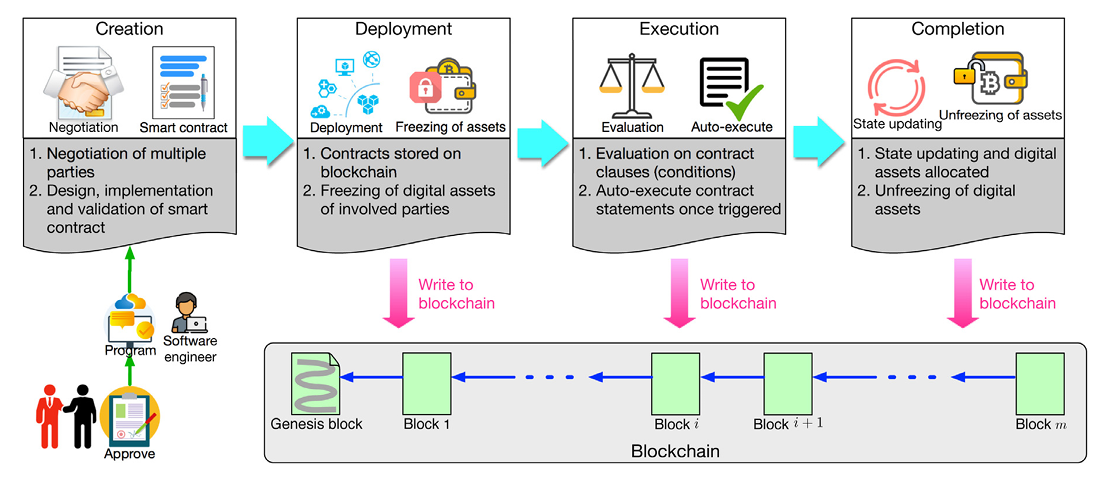
\includegraphics[width=0.7\textwidth]{resources/chapter-2/sc-lifecycle.png}
	\caption{\textit{Life cycle} dari Smart Contract \parencite{zheng2020overview}}
	\label{image:sc-lifecycle}
\end{figure}

\textit{Life cycle} dari sebuah Smart Contract terdiri dari empat fase seperti pada ilustrasi di Gambar \ref{image:sc-lifecycle}:

\begin{enumerate}
	\item \textit{Creation}: negosiasi antar pihak untuk menyepakati ketentuan dari kontrak dalam \textit{natural language}, dan translasi menjadi Smart Contracts.
	\item \textit{Deployment}: kontrak yang sudah divalidasi dapat disimpan ke dalam Blockchain, menjadikannya tidak bisa dimodifikasi.
	\item \textit{Execution}: Setelah \textit{deployment}, klausa kontraktual akan dimonitor, dan saat kondisi yang sesuai dengan yang terdefinisi dalam Smart Contract, maka prosedur kontrak akan dieksekusi secara otomatis.
	\item \textit{Completion}: Setelah eksekusi, \textit{state} baru dari semua pihak akan diperbarui sesuai dengan hasil dari transaksi yang terjadi dan disimpan ke dalam Blockchain. 
\end{enumerate}

\subsection{Off-Chain Smart Contracts}
\label{subsec:off-chain-smart-contracts}

\textit{Off-chain Smart Contract} adalah Smart Contracts yang dieksekusi diluar Blockchain, \textit{signed} hanya oleh \textit{interested participants}, dan digunakan untuk mengenkapsulasi fungsi yang melibatkan komputasi \textit{high-cost} atau \textit{private information} terkait \textit{participants}. Terdapat banyak cara untuk tetap menjaga properti dan keuntungan penggunaan dari Blockchain, contohnya, hasil dari eksekusi sebuah \textit{off-chain Smart Contract} dapat dilakukan \textit{logging} pada Blockchain, sehingga jika terjadi \textit{dispute} dalam eksekusi \textit{off-chain Smart Contract}, sebuah \textit{on-chain Smart Contract} dappat digunakan untuk \textit{fork off-chain Smart Contract} dan mengeksekusinya di dalam Blockchain untuk menyelesaikan \textit{dispute} \parencite{zou2019smart}.

\subsection{Semantic Smart Contracts}
\label{subsec:semantic-smart-contracts}
Semantic Smart Contracts adalah sebuah cara untuk merepresentasikan \textit{semantics} dari Smart Contract menggunakan konsep \textit{EthOn contract extension} dan sebuah \textit{vocabulary} yang terkait dengan bisnis. Semantic Smart Contracts mengizinkan untuk membandingkan \textit{request} dengan beberapa \textit{request description} dengan mengonsiderasi semantik dari anotasi yang mereferensikan sebuah \textit{shared domain ontology} \parencite{baqa2019semantic}.

\section{Ontology}
\label{sec:ontology}

Pada tahun 1993, \cite{gruber1993translation} pertama mendefinisikan sebuah ontology sebagai "\textit{explicit specification of a conceptualization}". Pada tahun 1997, \cite{borst1997construction} mendefinisikan ontology sebagai "\textit{formal specification of a shared conceptualization}". Definisi ini menambahkan kebutuhan sebuah ontology sebagai sebuah representasi konseptual yang \textit{shared} diantara beberapa pihak. Sehingga, konseptualisasi tersebut harus diekspresikan dengan sebuah format yang \textit{machine readable}. Sehingga pada tahun 1998, \cite{studer1998knowledge} menggabungkan kedua definisi tersebut sebagai "\textit{an ontology is a formal, explicit specification of a shared conceptualization}."

Dalam tulisannya, \cite{Guarino2009} merangkum ketiga definisi tersebut menjadi: Ontology adalah sebuah \textit{framework} terstruktur untuk merepresentasikan pengetahuan di sebuah \textit{domain} tertentu, seperti mendefinisikan entitas, konsep, dan relasi di dalam \textit{domain} tersebut. Ontology dapat membantu membuat sebuah model yang dapat dimengerti dan dapat dibagikan untuk digunakan dalam berbagai sistem dan aplikasi. Di dalam \textit{domain} sistem informasi, ontology digunakan sebagai sebuah cara formal untuk mengorganisasikan dan merepresentasikan data untuk dibagikan, dilakukan pencarian, dan dilakukan penalaran \parencite{Guarino2009}. 

Beberapa komponen kunci dari sebuah ontology adalah:

\begin{enumerate}
  \item \textit{Classes (Concepts)}: Tipe atau kategori fundamental di dalam sebuah \textit{domain} yang merepresentasikan konsep umum.
  \item \textit{Instances (Individuals)}: Contoh spesifik dari sebuah \textit{class}.
  \item \textit{Properties (Attributes)}: Mendeskripsikan karakteristik dari \textit{classes} atau \textit{instances}.
  \item \textit{Relationships}: Hubungan antar entitas, bisa \textit{hierarchical} atau \textit{associative}.
  \item \textit{Axioms}: Aturan atau \textit{constraint} yang mendefinisikan \textit{valid relationships} dan \textit{properties} di dalam ontology, sehingga dapat dilakukan inferensi logis.
\end{enumerate}

\subsection{The Semantic Web}
\label{subsec:the-semantic-web}

\textit{The Semantic Web} adalah sebuah ekstensi dari \textit{web} dengan tambahan data dengan arti yang terdefinisi dengan baik, yang diturunkan menggunakan \textit{semantic theory} untuk menginterpretasikan simbol-simbol. \textit{Semantic theory} menyediakan catatan dari arti untuk sebuah istilah atau informasi, sehingga dapat membuat sebuah hubungan logis antar istilah \parencite{shadbolt2006semantic}.

\subsubsection{Universal Resource Identifiers}
\label{subsubsec:universal-resource-identifiers}

\textit{Universal Resource Identifiers (URIs)} adalah sebuah cara untuk mengidentifikasi sebuah \textit{resource} menggunakan sebuah konvensi penamaan global yang disepakati, sehingga dapat diinterpretasikan secara standar oleh seluruh mesin yang berada di \textit{web}. Saat sebuah \textit{resource} diasosiasikan dengan sebuah URI, maka itu berarti semua orang dapat melakukan \textit{link}, \textit{refer}, dan mengambil \textit{representasi} dari \textit{resource} tersebut menggunakan URI. Skema yang direkomendasikan pada tahun 2004 adalah \textit{Resource Definition Framework Schema} yang menggunakan spesifikasi dasar dari RDF dengan ekstensi untuk mendukung ekspresi dari \textit{structured vocabularies} \parencite{shadbolt2006semantic}.

\subsubsection{Web Ontology Langugage}
\label{subsubsec:web-ontology-language}

Web Ontology Language (OWL) adalah keluarga bahasa yang dikembangkan oleh World Wide Web Consortium (W3C), digunakan untuk mengembangkan dan berbagi ontology di dalam \textit{web}. OWL bertujuan untuk memberikan representasi yang efisien untuk ontology, pengecekan \textit{logical consistency} dan klasifikasi \textit{concept}, menggunakan RDF untuk \textit{linking} sehingga ontology dapat didistribusikan antar sistem \parencite{shadbolt2006semantic}.

\subsection{Ontology in Blockchain}
\label{subsec:ontology-in-blockchain}

Konsep ontologi di dalam Blockchain adalah sebuah pendekatan yang berupaya untuk memetakan fitur dan konsep dari Blockchain secara formal dan \textit{shared} untuk mendukung \textit{interoperability} \parencite{9770809} dan mewujudkan visi \textit{semantic} Blockchain \parencite{hector2020blondie}. 

\subsubsection{EthOn}
\label{subsubsec:ethon}

\begin{figure}[ht]
  \centering
  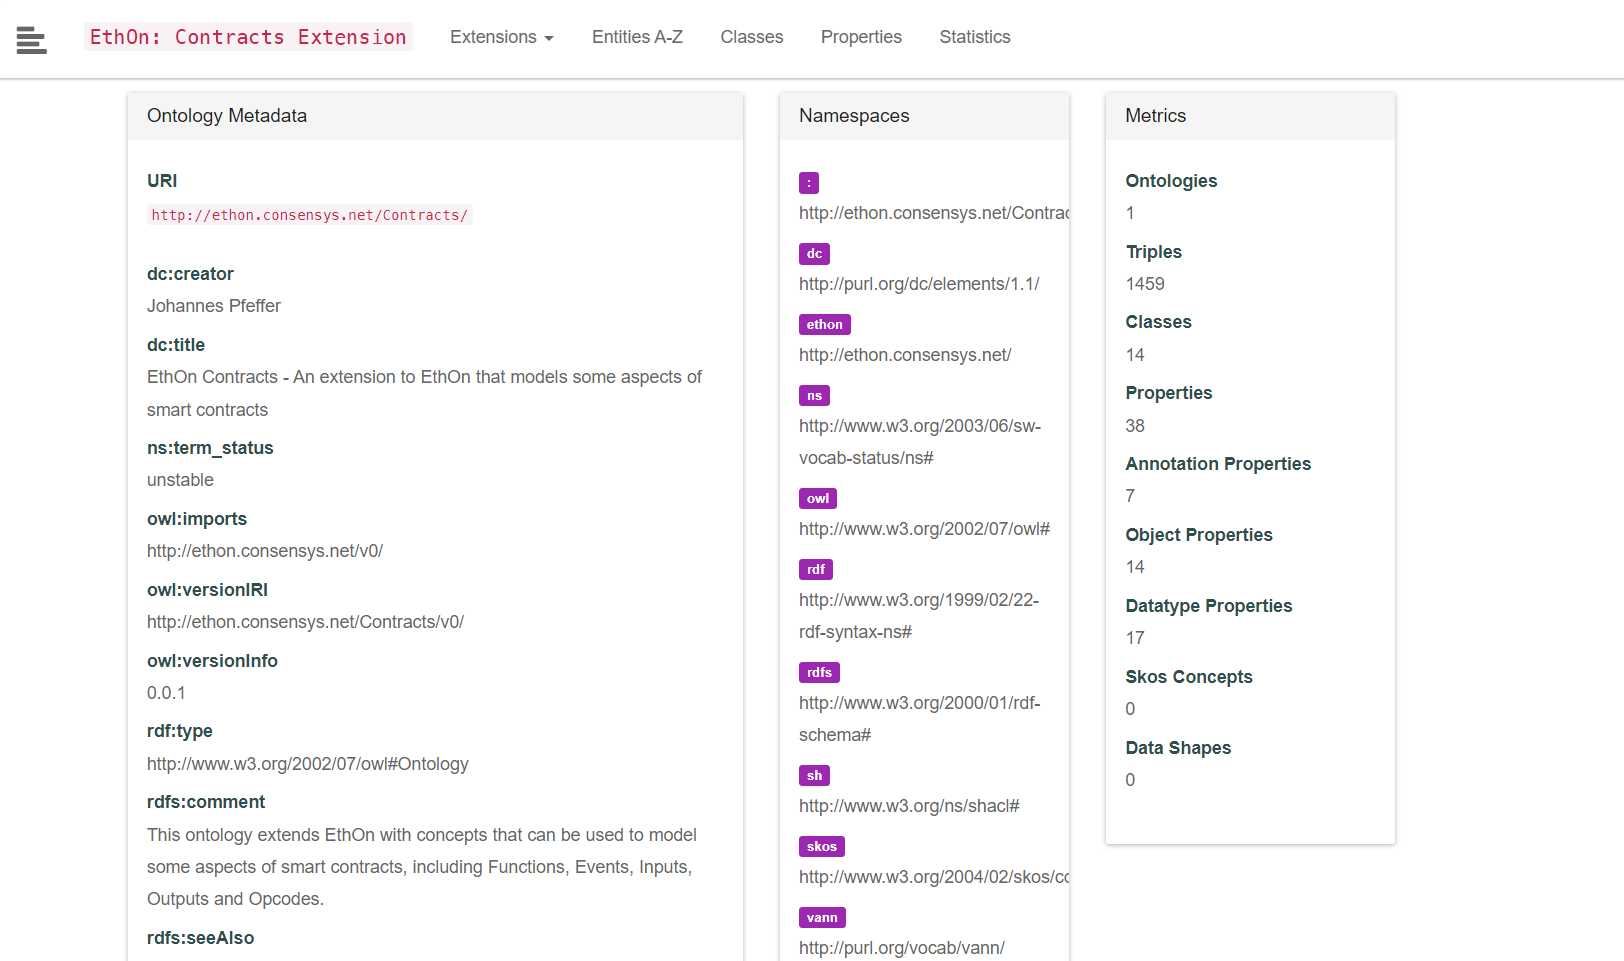
\includegraphics[width=0.7\textwidth]{resources/chapter-2/ethon.png}
  \caption{Visualisasi EthOn \parencite{ethon2024}}
  \label{image:ethon}
\end{figure}

EthOn adalah sebuah ontologi yang dirancang secara spesifik untuk ekosistem Ethereum untuk merepresentasikan struktur, komponen, dan relasi di dalam Blockchain Ethereum. EthOn menyediakan \textit{semantic framework} untuk standarisasi dan interpretasi data kompleks yang terasosiasi dengan transaksi, Smart Contracts, blok, akun, dan entitas lainnya. Ontology ini memberikan cara untuk menginterpretasikan data dengan cara yang lebih terstruktur dan berarti, mendukung \textit{interoperability}, dan integrasi data \parencite{pfeffer2016ethon}.

\subsubsection{BLONDiE}
\label{subsubsec:blondie}

\begin{figure}[ht]
  \centering
  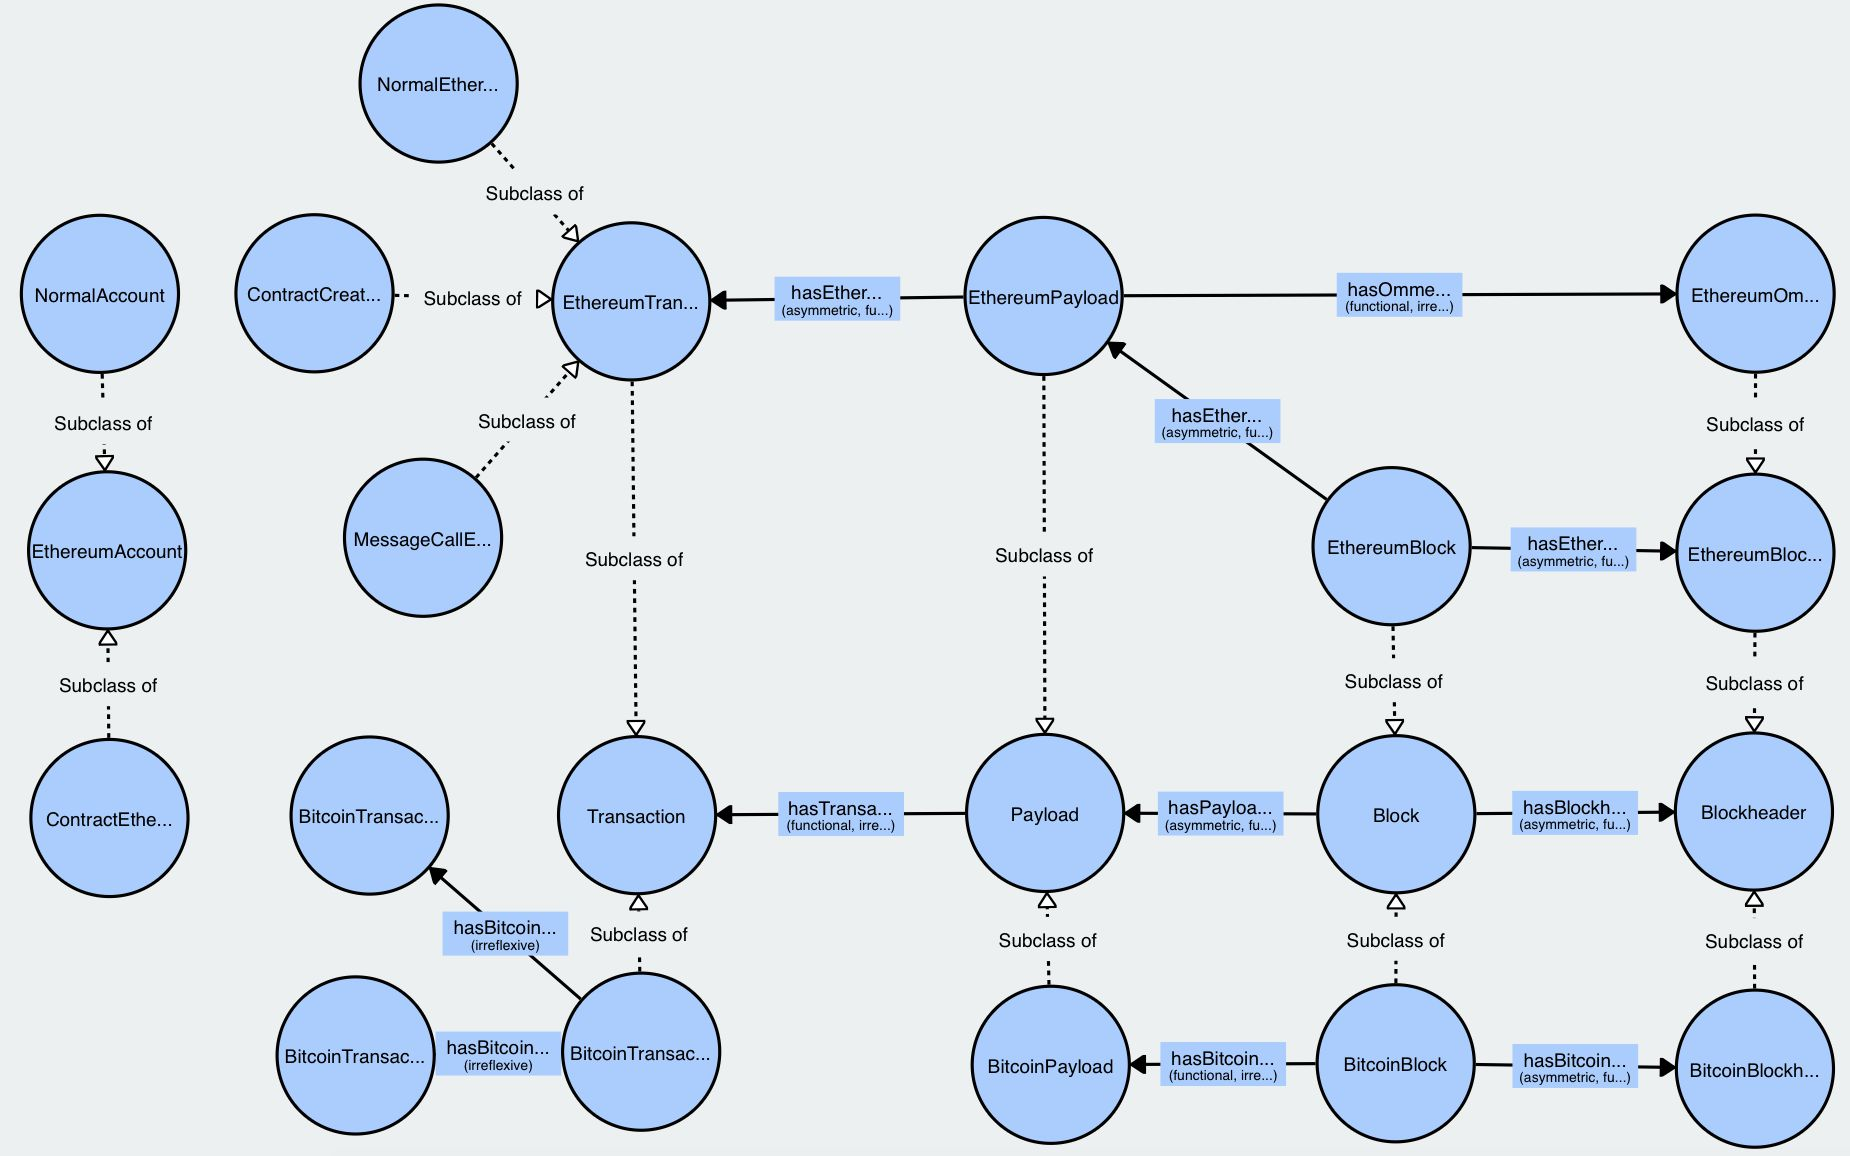
\includegraphics[width=1\textwidth]{resources/chapter-2/blondie-visualization.jpg}
  \caption{Visualisasi Ontologi BLONDiE \parencite{third2017linked}}
  \label{image:blondie-visualization}
\end{figure}

BLONDiE adalah singkatan dari Blockchain Ontology with Dynamic Extensibility, yang merupakan sebuah \textit{vocabulary} untuk merepresentasikan konsep di dalam Blockchain dengan potensi untuk ekstensi. Ontology ini terdiri atas 23 \textit{class}, 11 \textit{object properties}, dan 64 \textit{data properties} \parencite{hector2020blondie}. Gambar \ref{image:blondie-visualization} memvisualisasikan ontologi BLONDiE.

\subsection{Minimal Service Model}
\label{subsec:minimal-service-model}

Minimal Service Model adalah sebuah RDF(S) Integration Ontology sederhana berdasarkan prinsip \textit{minimal ontological commitment}, yaitu prinsip dalam perancangan ontology yang berarti membuat klaim atau asumsi sesedikit mungkin tentang domain yang dimodelkan. MSM hanya mendefinisikan struktur dasar seperti Services, Operations, dan Message Content. MSM dikembangkan bukan untuk menambah keragaman model \textit{service} yang sudah ada, melainkan berfungsi sebagai model untuk integrasi yang menjembatani berbagai formalisme yang telah ada. Model ini mampu menangkap semantik inti dari Web Service dan Web API dalam satu model yang sama, sehingga mendukung proses publikasi dan penemuan \textit{service} secara homogen. Salah satu fitur kunci dari MSM adalah kemampuan integrasinya, yang menggunakan properti msm untuk memungkinkan \textit{binding} ke berbagai format deskripsi untuk sebuah \textit{service} seperti WSDL, SWAGGER, WSMO, dan OWL-S, dan juga integrasi \textit{vocabulary} dari ontology lainnya \parencite{iserve2015datamodel}.

Ekstensi Minimal Service Model antara lain:
\begin{enumerate}
  \item MSM-WSDL \break Memberikan kemampuan \textit{grounding} ke elemen-elemen WSDL.
  \item MSM-SWAGGER \break Memberikan kemampuan \textit{grounding} untuk deskripsi SWAGGER.
  \item MSM-NFP \break Melacak metrik penggunaan \textit{service} yang mencakup informasi terkait properti non-fungsional.
\end{enumerate}

\begin{figure}[ht]
  \centering
  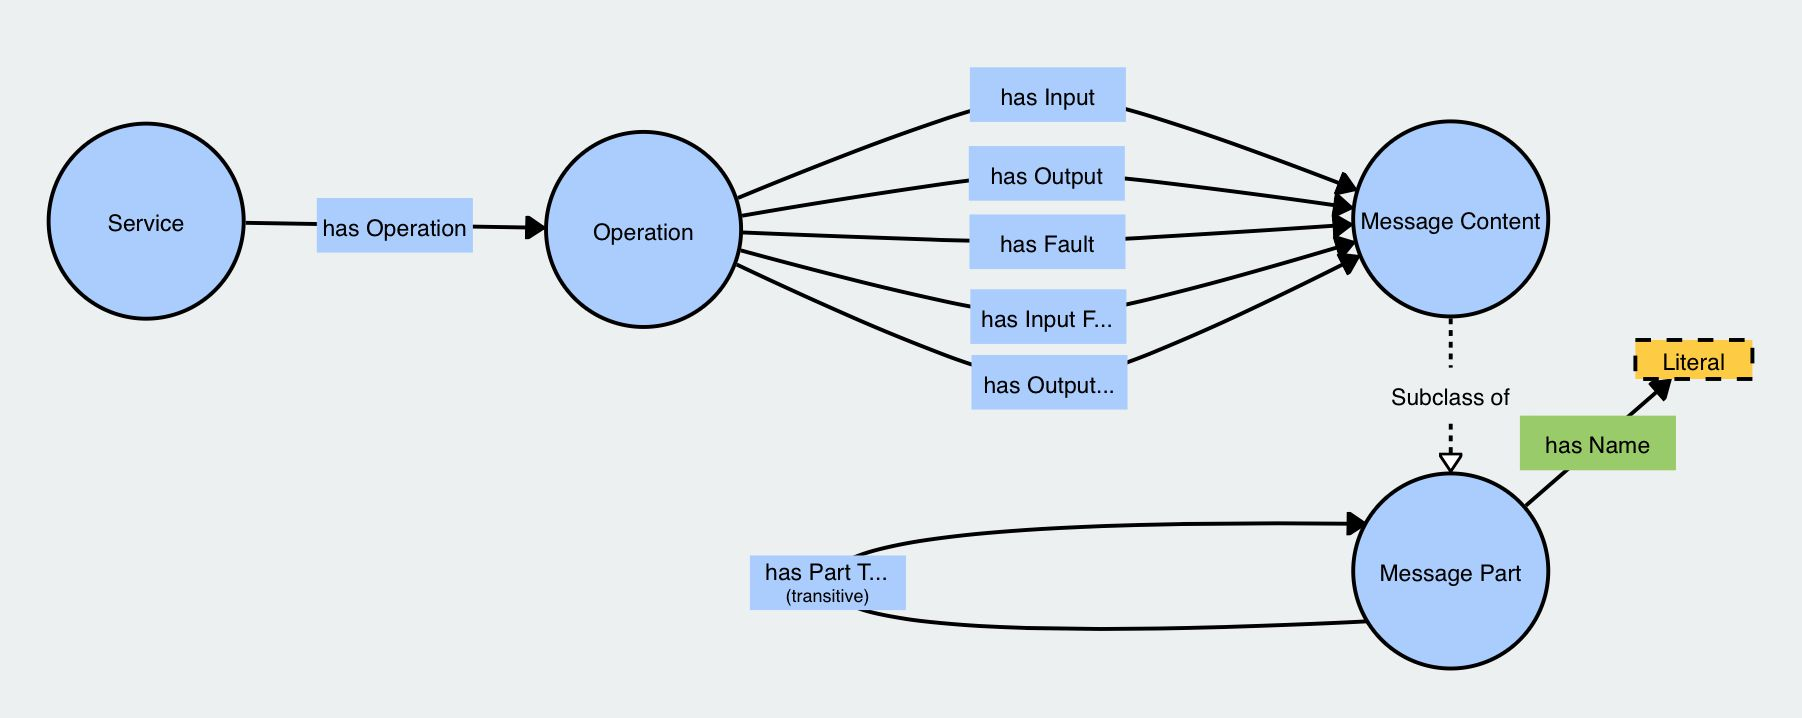
\includegraphics[width=1\textwidth]{resources/chapter-2/msm-visualization.jpg}
  \caption{Visualisasi Ontologi Minimal Service Model \parencite{third2017linked}}
  \label{image:msm-visualization}
\end{figure}
\section{Penelitian dan Riset Terkait}
\label{sec:penelitian-riset-terkait}

Berikut merupakan riset dan penelitian yang selaras dan juga menjadi komponen pendukung bagi tugas akhir ini.

% \subsection{RapidChain - Scaling Blockchain via Full Sharding}
\label{subsec:rapidchain}

RapidChain merupakan protokol blockchain publik berbasis \textit{sharding} pertama yang mampu mentoleransi \textit{Byzantine faults} sampai $\frac{1}{3}$ dari total partisipan, dan menggapai \textit{sharding} dari komunikasi, komputasi, dan \textit{overhead} penyimpanan secara menyeluruh. RapidChain menggunakan algoritma konsensus \textit{intra-committe} yang optimal sehingga dapat menggapai \textit{throughput} yang sangat tinggi menggunakan \textit{block pipelining}, \textit{novel gossiping protocol} untuk blok besar, dan mekanisme rekonfigurasi yang sudah terbukti aman untuk menjamin ketahanan. Untuk menghindari \textit{gossiping transactions} ke seluruh jaringan, RapidChain menggunakan teknik verifikasi transaksi \textit{cross-sharding} yang efisien.

RapidChain memberikan kebaruan sebagai berikut:

\begin{itemize}
  \item \textit{Sublinear Communication}
  \item \textit{Higher Resiliency}
  \item \textit{Rapid Committee Consensus}
  \item \textit{Secure Reconfiguration}
  \item \textit{Fast Cross-Shard Verification}
  \item \textit{Decentralized Bootstrapping}
\end{itemize}

RapidChain terdiri dari tiga komponen utama, yaitu \textit{Bootstrap}, \textit{Consensus}, dan \textit{Reconfiguration}. Protokol akan dimulai dengan fase \textit{Bootstrap}, dan dilanjutkan dengan menggunakan iterasi \textit{epoch}, dimana setiap \textit{epoch} akan terdiri dari beberapa iterasi dari \textit{Consensus} yang diikuti dengan fase \textit{Reconfiguration}.

Berikut merupakan penjelasan dari setiap fase:

\begin{enumerate}
  \item \textit{Bootstrapping}: Dalam fase ini, sebuah kelompok \textit{node} (\textit{root group}) menetapkan \textit{reference committee} dengan membangkitkan bit acak. \textit{Reference Committee} akan mengorganisasikan seluruh \textit{nodes} menjadi banyak \textit{committee} untuk pemrosesan transaksi secara paralel.
  \item \textit{Consensus in Committee}: Setiap \textit{committee} akan mengeksekusi protokol konsensus dua tahap. Tahap \textit{Gossiping Protocol (IDA-Gossip)}, yang membagikan \textit{message} besar menjadi bagian-bagian dan mendistribusikannya secara efisien antar \textit{node} menggunakan \textit{Merkle tree proofs}. Tahap kedua adalah tahap \textit{Synchrononous Consensus}, untuk memastikan resiliensi yang lebih tinggi dengan memperbolehkan \textit{committee} untuk berfungsi dengan jumlah \textit{honest node} (diatas 50\%), untuk meningkatkan resiliensi sistem keseluruhan menjadi $\frac{1}{3}$ \textit{faulty node}. 
  \item \textit{Cross-Shard Transactions}: \textit{Cross-Shard Transactions} memperbolehkan setiap \textit{node} untuk berinteraksi antar \textit{committee} berbeda sambil menyimpan hanya sebagian dari blockchain. \textit{Committees} menangani transaksi ini memanfaatkan verifikasi UTXO (\textit{Unspent Transaction Output}) di seluruh pecahan, yang mengurangi kebutuhan komunikasi dan penyimpanan dengan mengoordinasikan hanya informasi yang diperlukan.
  \item \textit{Inter-Committee Routing}: Memanfaatkan mekanisme \textit{routing} yang terinspirasi dari Kademlia, RapidChain memungkinkan \textit{node} untuk menemukan dan berkomunikasi satu sama lain di seluruh \textit{committee} dalam \textit{log-time steps}, yang memungkinkan verifikasi transaksi tanpa memerlukan pesan "\textit{gossip-to-all}". 
  \item \textit{Reconfiguration}: \textit{Reconfiguration} periodik memastikan bahwa \textit{node} diacak dengan aman di seluruh \textit{committee} menggunakan aturan Cuckoo untuk melindungi dari kontrol yang berlawanan. Fase ini memungkinkan \textit{node} baru untuk bergabung tanpa mengganggu operasi protokol yang sedang berlangsung.
\end{enumerate}

\subsection{Linked Data Indexing of Distributed Ledgers}
\label{subsec:linked-data-indexing-distributed-ledgers}

Penelitian yang dilakukan oleh \cite{third2017linked} membahas tantangan dalam pencarian informasi pada \textit{distributed ledger}, yang sulit dilakukan karena informasi mengenai suatu entitas dapat tersebar di seluruh \textit{ledger} tanpa adanya indeks. Penelitian ini mengusulkan penggunaan indeks berbasis semantik untuk Ethereum Blockchain dengan pendekatan \textit{Linked Data}, yang memungkinkan pencarian menggunakan istilah khusus sesuai \textit{domain}. Pendekatan ini diharapkan dapat meningkatkan kekuatan, kegunaan, dan cakupan dari sistem \textit{ledger} tersebut.

Dalam penelitian ini, mereka mengimplementasikan indeks semantik pada Ethereum Blockchain untuk mengekspos data di dalam \textit{distributed ledger} sebagai \textit{Linked Data}. Indeks ini mengindeks data pada level blok dan transaksi menggunakan ontologi BLONDiE, serta memetakan Smart Contract ke dalam ontologi \textit{Minimal Service Model} (MSM) sebagai langkah awal untuk menghubungkan Smart Contract dengan \textit{Semantic Web Services}.

Implementasi indeks semantik ini menggunakan ontologi BLONDiE sebagai kerangka untuk mengelompokkan dan mendeskripsikan elemen-elemen utama dari Blockchain. Ontologi \textit{Minimal Service Model}, yang biasanya digunakan untuk \textit{web services}, diterapkan untuk menggambarkan fungsionalitas dari Smart Contract pada Blockchain, sehingga memungkinkan integrasi yang lebih efisien.

\begin{figure}[ht]
  \centering
  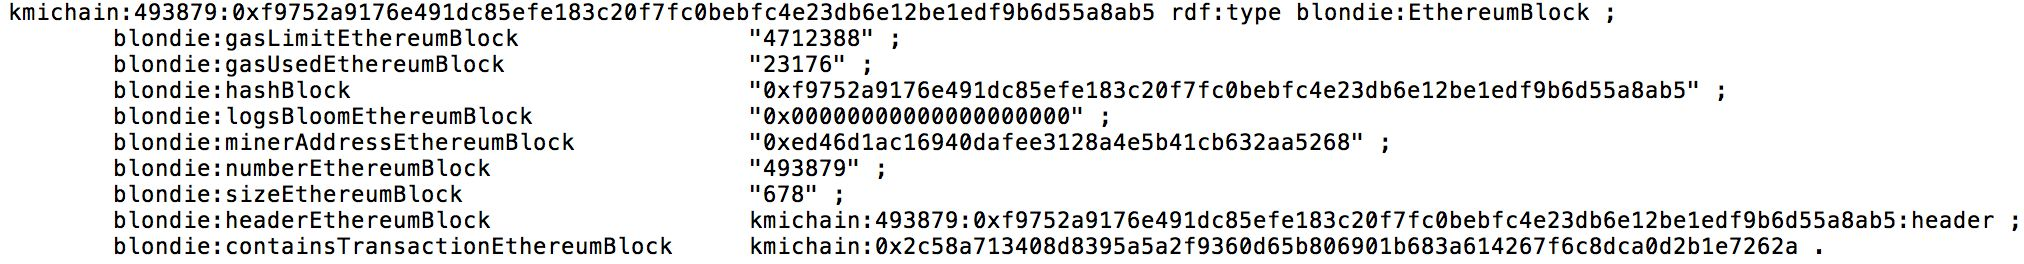
\includegraphics[width=1\textwidth]{resources/chapter-2/rdf-block.jpg}
  \caption{RDF dari deskripsi blok \parencite{third2017linked}}
  \label{image:rdf-block}
\end{figure}

\begin{figure}[ht]
  \centering
  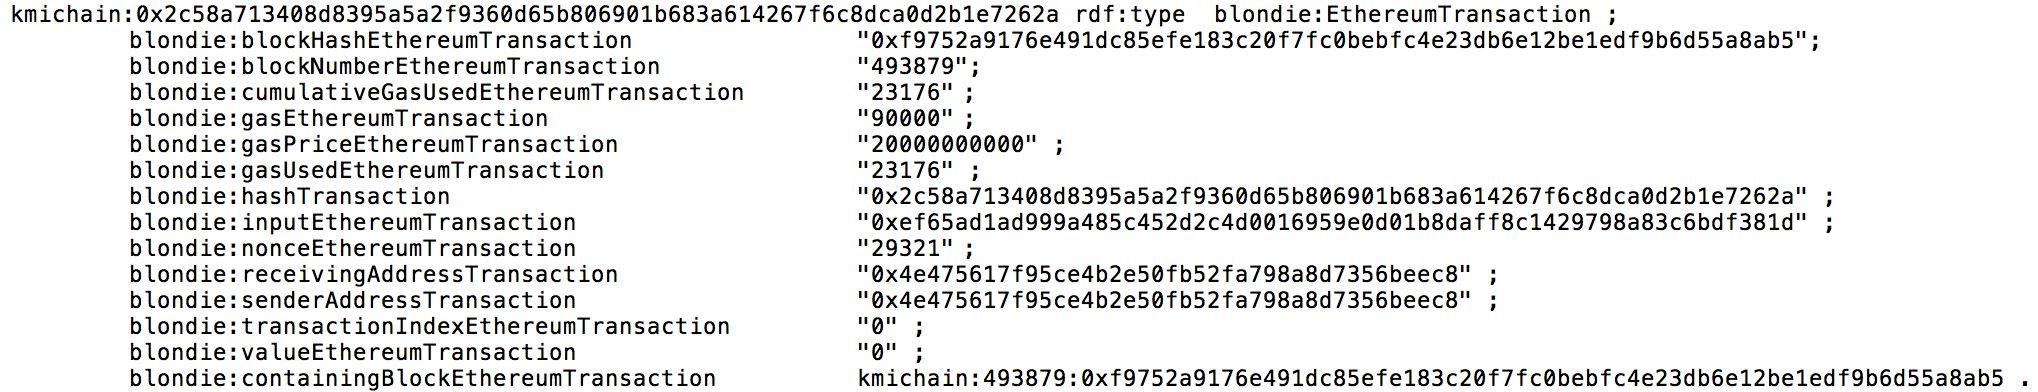
\includegraphics[width=1\textwidth]{resources/chapter-2/rdf-transaction.jpg}
  \caption{RDF dari deskripsi transaksi \parencite{third2017linked}}
  \label{image:rdf-transaction}
\end{figure}

Proyek ini diimplementasikan pada jaringan Ethereum Blockchain privat, di mana komponen \textit{listener} dikembangkan untuk mendeteksi blok baru dan mengindeksnya berdasarkan ontologi BLONDiE. RDF \textit{triples} kemudian dihasilkan dari data ini, yang memungkinkan penguraian data Blockchain secara semantik untuk mendukung pencarian data yang lebih terstruktur. Gambar \ref{image:rdf-block} dan gambar \ref{image:rdf-transaction} adalah contoh dari RDF \textit{triples} yang dihasilkan dari deskripsi blok dan transaksi masing-masing.

Hasil dari penelitian ini menunjukkan bahwa \textit{semantic indexing} memungkinkan data di dalam Blockchain menjadi lebih mudah diakses dan dapat terintegrasi dengan sumber data eksternal. Hal ini membuka peluang untuk mengembangkan \textit{semantic indexing} pada platform Blockchain lainnya serta berpotensi memperluas interoperabilitas data antara Blockchain dan \textit{Semantic Web}.
\subsection{Extraction, indexing, and analysis of Ethereum Smart Contracts data}
\label{subsec:extraction-indexing-analysis-ethereum-sc}

\begin{figure}[ht]
	\centering
	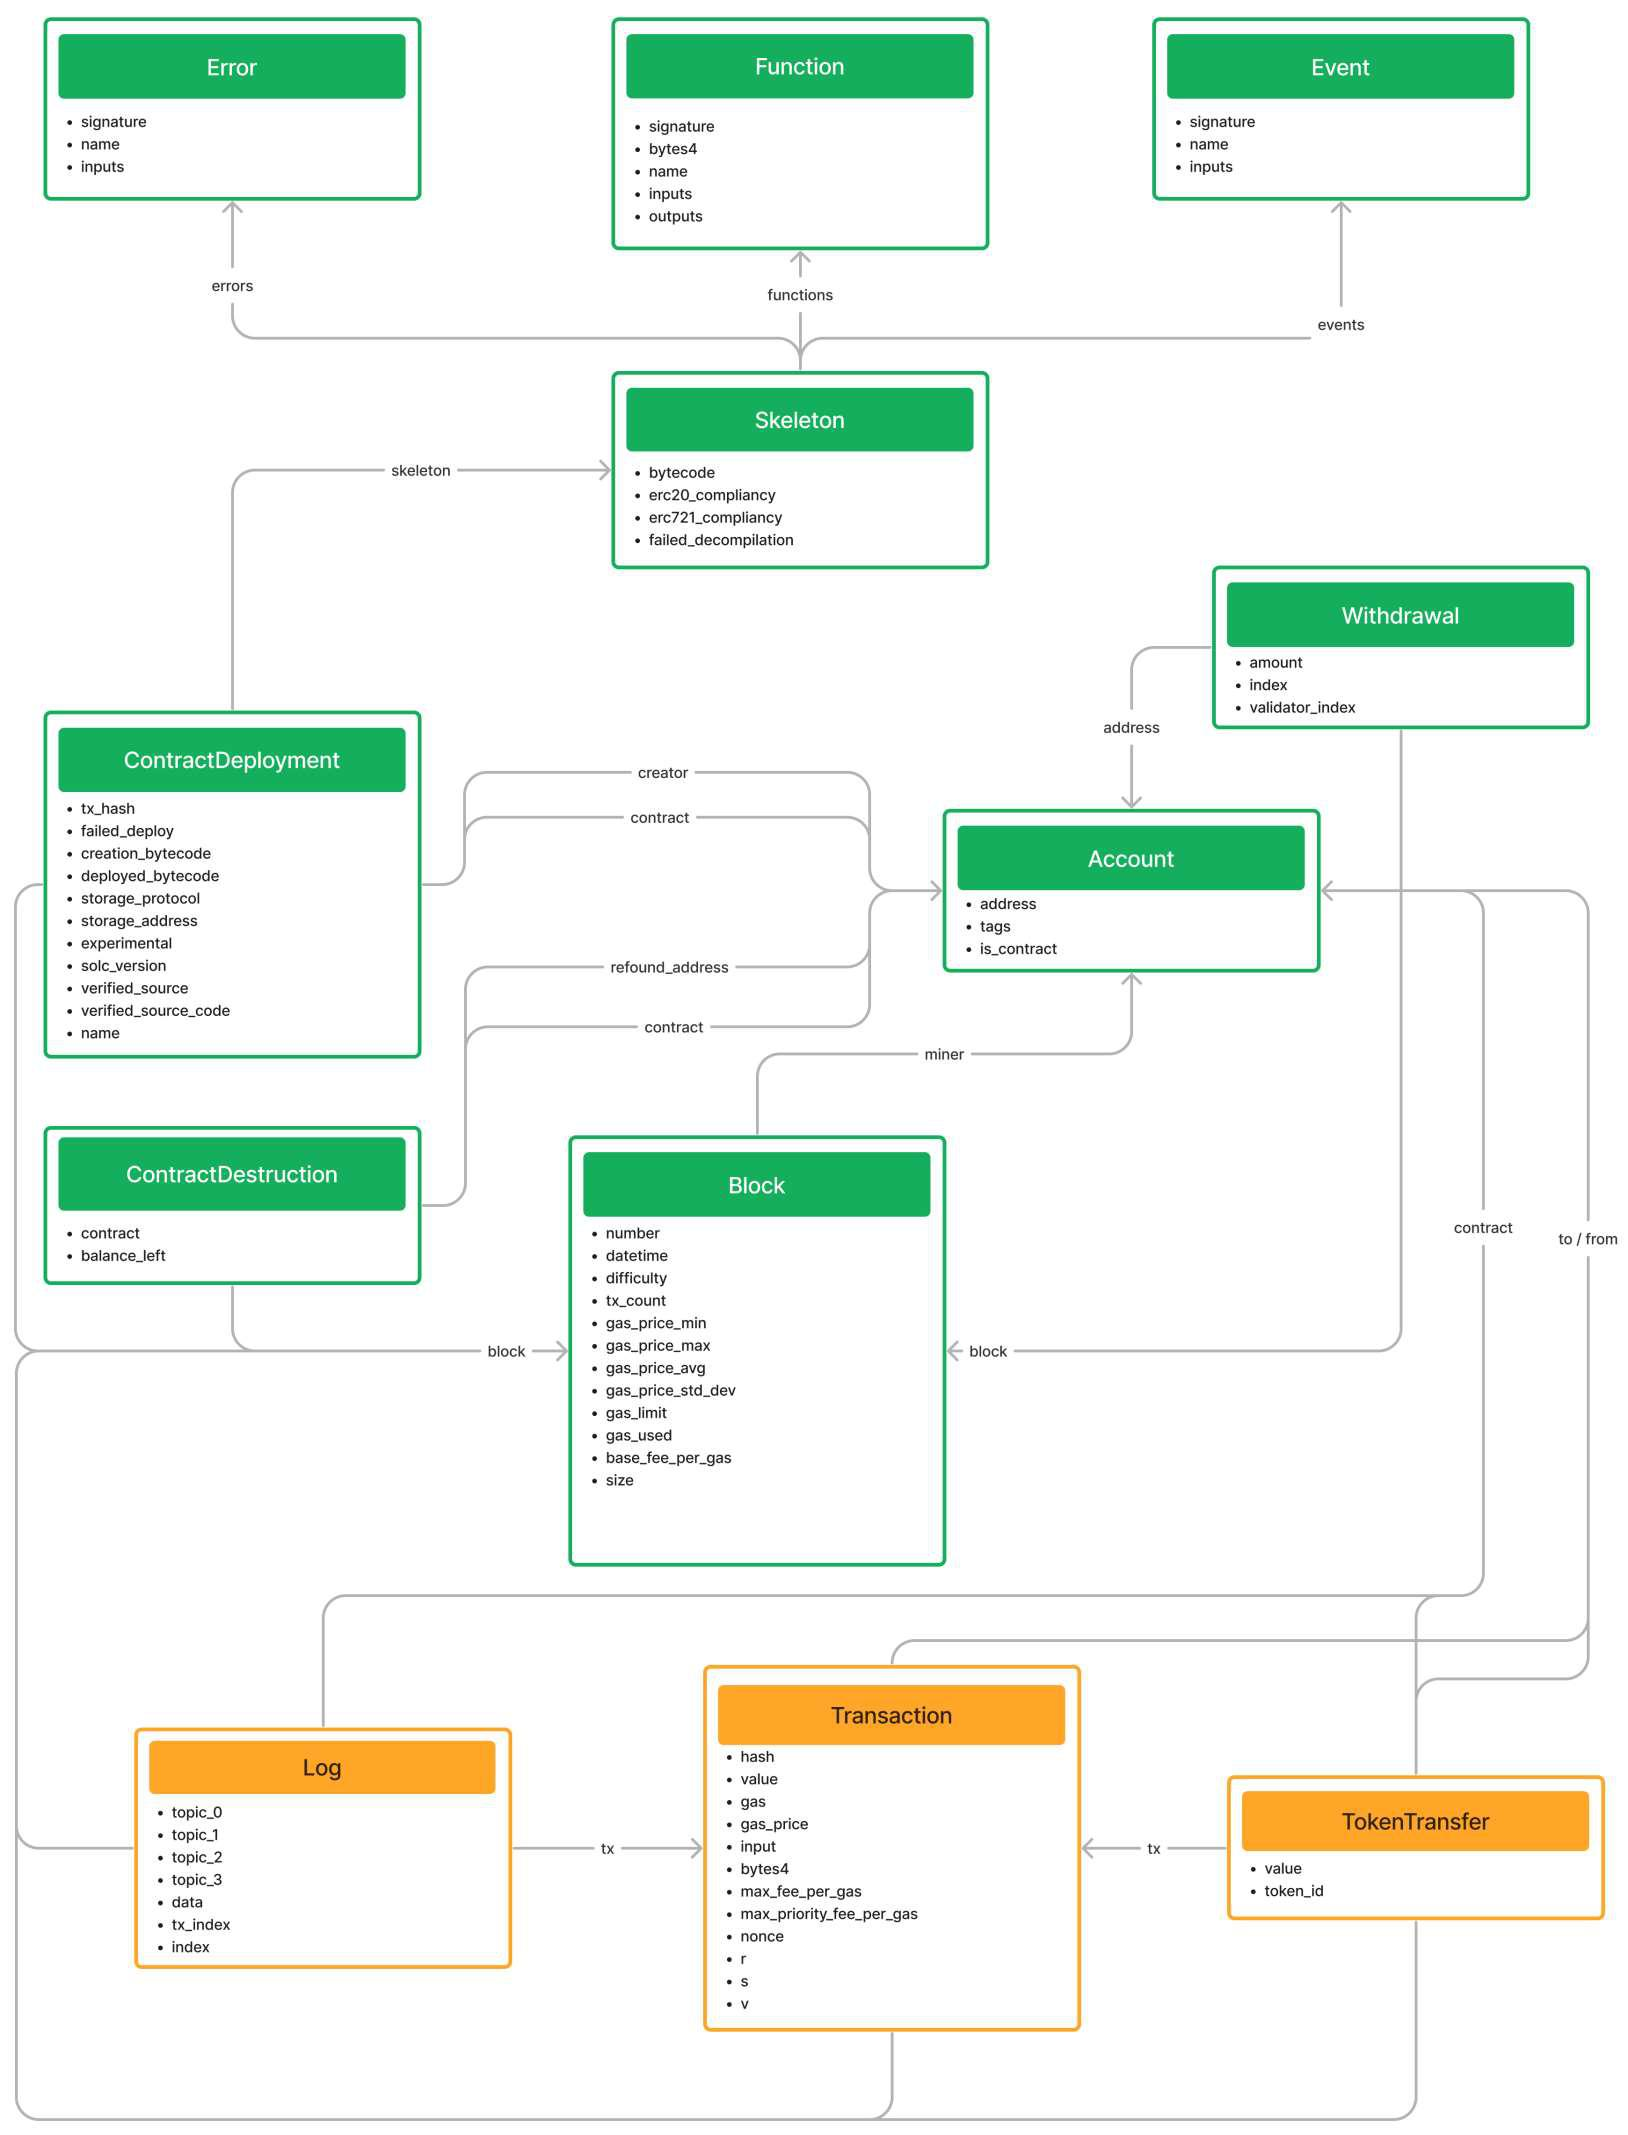
\includegraphics[width=0.7\textwidth]{resources/chapter-2/eth2dgraph-structure.jpg}
	\caption{Data model eth2dgraph \parencite{aimar2023extraction}}
	\label{image:eth2dgraph-structure}
\end{figure}

Penelitian yang dilakukan sebagai \textit{thesis} oleh \cite{aimar2023extraction} berfokus pada bagaimana mengambil data dari Blockchain Ethereum yang bersifat publik, mengekstrasi semantiknya, lalu mentransformasikannya ke sebuah bentuk yang mudah diakses oleh pengguna dengan cara mengindeksnya menggunakan Dgraph, sebuah \textit{open-source distributed graph database}. Hasil dari penelitian ini adalah sebuah perangkat lunak bernama eth2dgraph, yang ditulis dalam bahasa Rust yang melakukan mapping data Ethereum ke format Dgraph, dengan data model yang ditunjukkan pada gambar \ref{image:eth2dgraph-structure}. Perangkat lunak ini mengintegrasikan sebuah \textit{decompiler} untuk mengekstraksi dan mengindeks ABI dari Smart Contracts.

Beberapa hal yang dapat diperhatikan dari perangkat lunak eth2dgraph adalah:

\begin{enumerate}
	\item Ekstraksi ABI \newline Cara eth2dgraph mengekstraksi semantik dari sebuah Smart Contract yang sudah dalam bentuk EVM Bytecode, yaitu dalam ABI (\textit{Application Binary Interface}). Gambar \ref{image:abi-extraction} menggambarkan bagaimana eth2dgraph memanfaatkan heimdall-rs untuk melakukan dekompilasi ABI. Cara ini dapat mengekstraksi lokasi fungsi, informasi terkait tipe \textit{input} dan \textit{output} dan nama fungsi, tetapi tidak memungkinkan untuk mengekstraksi nama parameter karena sudah dihilangkan pada saat kompilasi.
	      \begin{figure}[ht]
		      \centering
		      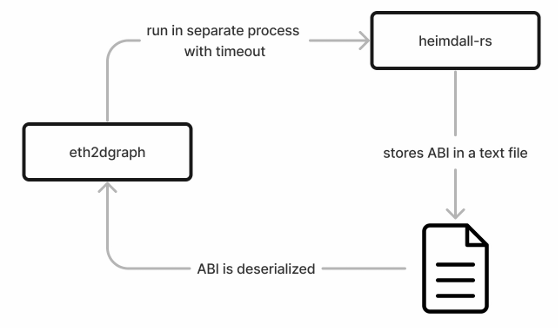
\includegraphics[width=0.7\textwidth]{resources/chapter-2/eth2dgraph-heimdall.png}
		      \caption{Ekstraksi ABI \parencite{aimar2023extraction}}
		      \label{image:abi-extraction}
	      \end{figure}
	\item Ekstraksi struktur dan metadata \newline Cara eth2dgraph mengekstraksi struktur Smart Contract dan metadata adalah menggunakan Regular Expression, dengan bagian \textit{runtime} diproses untuk mengekstraksi struktur, sedangkan bagian metadata dilakukan \textit{decode}.
	\item Ekstraksi menggunakan source code \newline eth2dgraph juga dapat melakukan ekstraksi semantik menggunakan source code yang tersedia dari sebuah Smart Contract, dengan cara melakukan query terhadap teks yang ada di dalam Smart Contract.
\end{enumerate}

\subsection{Semantic Smart Contracts for Blockchain-based Services in the Internet of Things}
\label{subsec:semantic-smart-contract-iot}

Penelitian yang dilakukan oleh \cite{baqa2019semantic}, mengusulkan sebuah solusi untuk menemukan dan menggunakan Smart Contract untuk kegunaan spesifik, yang sulit dilakukan karena Smart Contract biasanya sudah dikompilasi dalam bentuk \textit{byte-code}, tanpa metadata yang terasosiasi. Solusi yang diusulkan adalah Semantic Smart Contract yang mengintegrasikan RESTful Semantic Web Technologies dalam Smart Contract, yang di-\textit{deploy} pada Blockchain Ethereum untuk melakukan \textit{indexing}, \textit{browsing}, dan melakukan anotasi terhadap sebuah Smart Contract. Penelitian ini menggunakan penelitian \cite{third2017linked} terkait Linked Data Indexing untuk meningkatkan \textit{discoverability}.

\begin{figure}[ht]
	\centering
	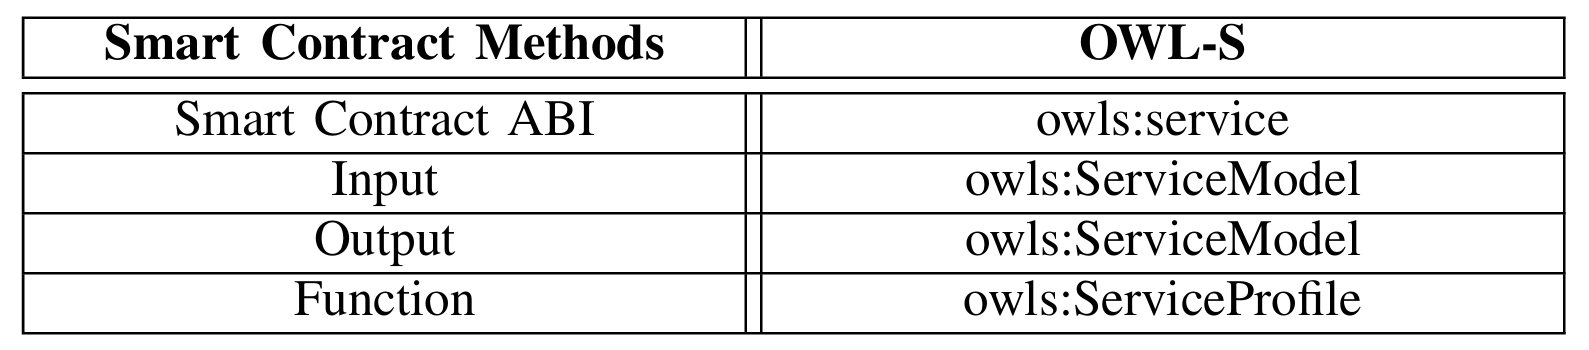
\includegraphics[width=0.7\textwidth]{resources/chapter-2/ssc-ontology-extension.png}
	\caption{Ekstensi OWL-S \parencite{baqa2019semantic}}
	\label{image:ekstensi-owl-s}
\end{figure}

Dalam pengembangan solusi yang diusulkan dalam penelitian ini, dilakukan ekstensi pada OWL-S Service Ontology, seperti pada gambar \ref{image:ekstensi-owl-s} dengan menginkorporasikan beberapa terminologi yang \textit{domain specific} seperti yang ada di dalam EthOn. Sehingga, Semantic Smart Contract dapat digunakan untuk memperkaya query untuk sebuah terminologi yang \textit{domain specific} antar beberapa \textit{distributed ledgers}, yang meningkatkan \textit{discoverability} dari sebuah aplikasi IoT yang terdesentralisasi.
\subsection{Ontological Modeling of Smart Contracts in Solidity}
\label{subsec:solidity-ontology}

Formalisasi menggunakan ontology berbasis domain baru dilakukan pada Blockchain dan Smart Contract, tetapi belum ada yang dilakukan terhadap bahasa pemrograman Smart Contract itu sendiri. Pada penelitiannya, \cite{cano2021toward} mengusulkan sebuah representasi dari bahasa pemrograman Smart Contract yang terkemuka, yaitu Solidity, dengan mendefinisikan semua entitas yang dibutuhkan untuk mencakup seluruh bahasa dan menyelaraskan ke ontology terstandarisasi lainnya seperti EthOn.

Beberapa spesifikasi yang dituliskan di dalam penelitian ini:

\begin{enumerate}
  \item Implementasi Solidity Library
  \item Implementasi Solidity Contract
  \item Interface dan Abstract Contract Solidity
  \item Spesifikasi Attributes dan representasinya di dalam Ontology 
  \item Spesifikasi Types dan representasinya di dalam Ontology
  \item Spesifikasi Constructor dan representasinya di dalam Ontology
  \item Spesifikasi Function dan representasinya di dalam Ontology
  \item Spesifikasi Modifier dan representasinya di dalam Ontology
  \item Spesifikasi Receive dan representasinya di dalam Ontology
  \item Spesifikasi Fallback dan representasinya di dalam Ontology
  \item Spesifikasi Event dan representasinya di dalam Ontology
\end{enumerate}


% Bab Studi Literatur digunakan untuk mendeskripsikan kajian literatur yang terkait dengan persoalan tugas akhir. Tujuan studi literatur adalah:

% \begin{enumerate}
% 	\item menunjukkan kepada pembaca adanya gap seperti pada rumusan masalah yang memang belum terselesaikan,
% 	\item memberikan pemahaman secukupnya kepada pembaca tentang teori atau pekerjaan terkait yang terkait langsung dengan penyelesaian persoalan, serta
% 	\item menyampaikan informasi apa saja yang sudah ditulis/dilaporkan oleh pihak lain (peneliti/Tugas Akhir/Tesis) tentang hasil penelitian/pekerjaan mereka yang sama atau mirip kaitannya dengan persoalan tugas akhir.
% \end{enumerate}

% Kita juga dapat memisah beberapa bagian latex untuk \textit{readability}. Kita dapat memasukan file latex lainnya dengan menggunakan fitur input. Berikut merupakan contoh ketika memasukan bagian contoh-subbab ke chapter-2


% \section{Menyisipkan Persamaan}

% Beberapa contoh menyisipkan persamaan.

% \subsection{Contoh Bikin Equation}
% \textbf{text tebal} dan ini \emph{miring}, bikin persamaan di baris yang sama, tinggal pake dolar2 $\Psi(\vec{r}_1,...,\vec{r}_N)$, sehingga persamaan Schr\"{o}dinger, terus, persamaan yang dinomeri kayak gini
% %ini contoh bikin persamaan, ..... :D
% \begin{equation}
% 	\left[ \sum_{i}^{N}-\frac{\hbar^2}{2m}\nabla_i^2 + \sum_{i}^{N}V(\vec{r}_i)+ \sum_{i<j}^{N}(\vec{r}_i,\vec{r}_j)\right]\Psi = E\Psi
% \end{equation}

% untuk $N$-elektron, dengan $\hat{H}$=Hamiltonian, $E$=Energi total, $\hat{T}$=Energi kinetik, $\hat{V}$=Energi potensial, dan $\hat{U}$=Interaksi ektron-elektron.

% \subsection{Bikin Matrix}
% Lalalallala.... bikin matrix sekarang, yang ini dikecilin, pake smaller
% 	{\smaller
% 		\begin{equation}
% 			\Psi({\bf r}_1, {\bf r}_2, \cdots {\bf r}_N) = \frac{1}{\sqrt{N!}}\left| \begin{array}{llcl}
% 				\phi_1({\bf r}_1)     & \phi_2({\bf r}_1)     & \cdots                & \phi_N({\bf r}_1)     \\
% 				\phi_1({\bf r}_2)     & \phi_2({\bf r}_2)     & \cdots                & \phi_N({\bf r}_2)     \\
% 				\phi_1({\bf r}_3)     & \phi_2({\bf r}_3)     & \cdots                & \phi_N({\bf r}_3)     \\
% 				\multicolumn{1}{c}{.} & \multicolumn{1}{c}{.} & \multicolumn{1}{c}{.} & \multicolumn{1}{c}{.} \\
% 				\multicolumn{1}{c}{.} & \multicolumn{1}{c}{.} & \multicolumn{1}{c}{.} & \multicolumn{1}{c}{.} \\
% 				\multicolumn{1}{c}{.} & \multicolumn{1}{c}{.} & \multicolumn{1}{c}{.} & \multicolumn{1}{c}{.} \\
% 				\phi_1({\bf r}_N)     & \phi_2({\bf r}_N)     & \cdots                & \phi_N({\bf r}_N)     \\
% 			\end{array} \right|
% 		\end{equation}
% 	}